\begin{enumerate}[label=\thechapter.\arabic*,ref=\thechapter.\theenumi]
\item
For the circuit given below, choose the angular frequency $ \omega_0$ at which voltage across capacitor has maximum amplitude?
\begin{figure}[h!]
    \includegraphics[width = 0.5\columnwidth]{2023/BM/16/figs/c_fig1.pdf}
    \caption{circuit }
    \centering
    \label{fig: bm_16_fig_1}
\end{figure}
\begin{enumerate}
    \item[(A)] 1000
    \item[(B)] 100
    \item[(C)] 1
    \item[(D)] 0   
\end{enumerate}
\hfill(GATE BM 2023 Question 16)\\

\solution
\input{2023/BM/16/asnmt3.tex}
\newpage
\item
In the following circuit, the switch S is open for $t < 0$ and closed for $t \ge 0$.
What is the steady state voltage (in Volts) across the capacitor when the switch is closed?
\begin{figure}[h!]
    \includegraphics[width = 0.7\columnwidth]{2023/BM/30/figs/c_fig1.pdf}
    \caption{circuit }
    \centering
    \label{fig:bm_30_fig_1}
\end{figure}
\hfill(GATE BM 2023 Question 30) \\
\solution
\input{2023/BM/30/main.tex}
\pagebreak
\item 
A finite impulse response (FIR) filter has only two non-zero samples in its impulse response $h[n]$, namely $h[0] = h[1] = 1$. The Discrete Time Fourier Transform (DTFT) of $h[n]$ equals $H(e^{j\omega})$, as a function of the normalized angular frequency $\omega$. For the range $\abs{\omega} \leq \pi$, $\abs{H(e^{j\omega})}$ is equal to
\begin{enumerate}
	\item[(A)] $2\abs{\cos(\omega)}$
	\item[(B)] $2\abs{\sin(\omega)}$
	\item[(C)] $2\abs{\cos(\frac{\omega}{2})}$
	\item[(D)] $2\abs{\sin(\frac{\omega}{2})}$
\end{enumerate}
\hfill(GATE BM 2023 Question 17) \\
\solution
\input{2023/BM/17/1.tex}
\pagebreak
\item
For the circuit shown,if $i=\sin 1000t$, the instantaneous value of the Thevenin's voltage(in volts) across the terminals a anb b at time t=5ms is\\[2pt]

\begin{circuitikz}[american voltages,american currents]
    % Draw the circuit components
    \draw (0,0) -- (2,0);
    \draw (2,2) to [resistor,l=$10\Omega$] (2,4);
    \draw (2,4) -- (0,4);
    \draw (2,0) to [capacitor,l=$-j10\Omega$,-,i_=$i_x$] (2,2);
    \draw (2,0) -- (5,0);
    \draw (5,0) to[inductor,l=$j10\Omega$] (5,2);
    \draw (5,2) to [resistor,l=$10\Omega$] (5,4);
  \draw (5,4) to [cV,l^=$4i_x$,invert] (2,4);
  \draw (5,4) -- (6,4);
  \draw (6,4) to[I,l=$\sin 1000t$,invert] (6,0);
  \draw (6,0) -- (5,0);
   \node[circle,fill=black,inner sep=1.5pt,label=above:a] at (0,0) {};
    \node[circle,fill=black,inner sep=1.5pt,label=above:b] at (0,4) {};
    \end{circuitikz}
    \hfill(GATE EE 2023 ) \\
    \solution
    \input{2023/EE/51/gate51.2023.tex}
    \pagebreak

    \item In the circuit shown ,$\omega=100\pi\text{rads/s}$, R1=R2=$2.2\Omega$ and L=$7\text{mH}$. the capacitance $\text{C}$ for which $Y_{in}$ is purely real is  $\text{mF}$ \\
	\begin{center}
	\begin{circuitikz} \centering \draw 
		(0,4) to[sinusoidal voltage source, l=$V_{0}$cos($\omega$t)] (0,0)
		(0,4) to[short] (4,4)
		(4,4) to[resistor, l=$R_1$ ] (4,2)
		(4,2) to[inductor, l= $\text{L} $] (4,0) to[short ] (0,0)
		(8,4)  to[short] (4,4)
		(8,4) to[resistor, l= $R_2$] (8,2) to[capacitor,l=$\text{C}$] (8,0) to (4,0);
	\end{circuitikz}
	\end{center}
\hfill(GATE IN 2023 Q46)\\
\solution
\input{2023/IN/46/7.tex}

\pagebreak
\item An input voltage in the form of a square wave of frequency $1\, kHz$ is given to a circuit, which results in the output shown schematically below. Which one of the following options is the CORRECT representation of the circuit? \hfill(GATE PH 2023 Q37)
\begin{figure}[!h]
    \centering
    \includegraphics[width = 0.6\columnwidth]{2023/PH/37/figs/question.png}
	\caption{}\
	\label{fig:ques_gate.ph.23.37}
\end{figure}

\begin{enumerate}[label = (\alph*)]
    \item 
    \begin{figure}[!h]
        \centering
	    \resizebox{0.2\textwidth}{!}{\input{2023/PH/37/figs/optA}}
	\label{optA_gate.ph.23.37}
    \end{figure}

    \item 
    \begin{figure}[!h]
        \centering
        \resizebox{0.2\textwidth}{!}{\input{2023/PH/37/figs/optB}}
        \label{optB_gate.ph.23.37}
    \end{figure}

    \item 
    \begin{figure}[!h]
        \centering
        \resizebox{0.2\textwidth}{!}{\input{2023/PH/37/figs/optC}}
        \label{optC_gate.ph.23.37}
    \end{figure}

    \item 
    \begin{figure}[!h]
        \centering
        \resizebox{0.2\textwidth}{!}{\input{2023/PH/37/figs/optD}}
        \label{optD_gate.ph.23.37}
    \end{figure}
\end{enumerate} \hfill(GATE 2023 PH 37)\\
\solution
\input{2023/PH/37/GATE_PH_23_37.tex}
\pagebreak

\item In the circuit shown below, switch S was closed for long time. If the switch is opened at $t=0$, the  maximum magnitude of the voltage $V_R$ , in volts is (rounded off to the nearest integer)\hfill{(GATE 2023 EC 35)}\\
\begin{figure}[h!]
    \centering
    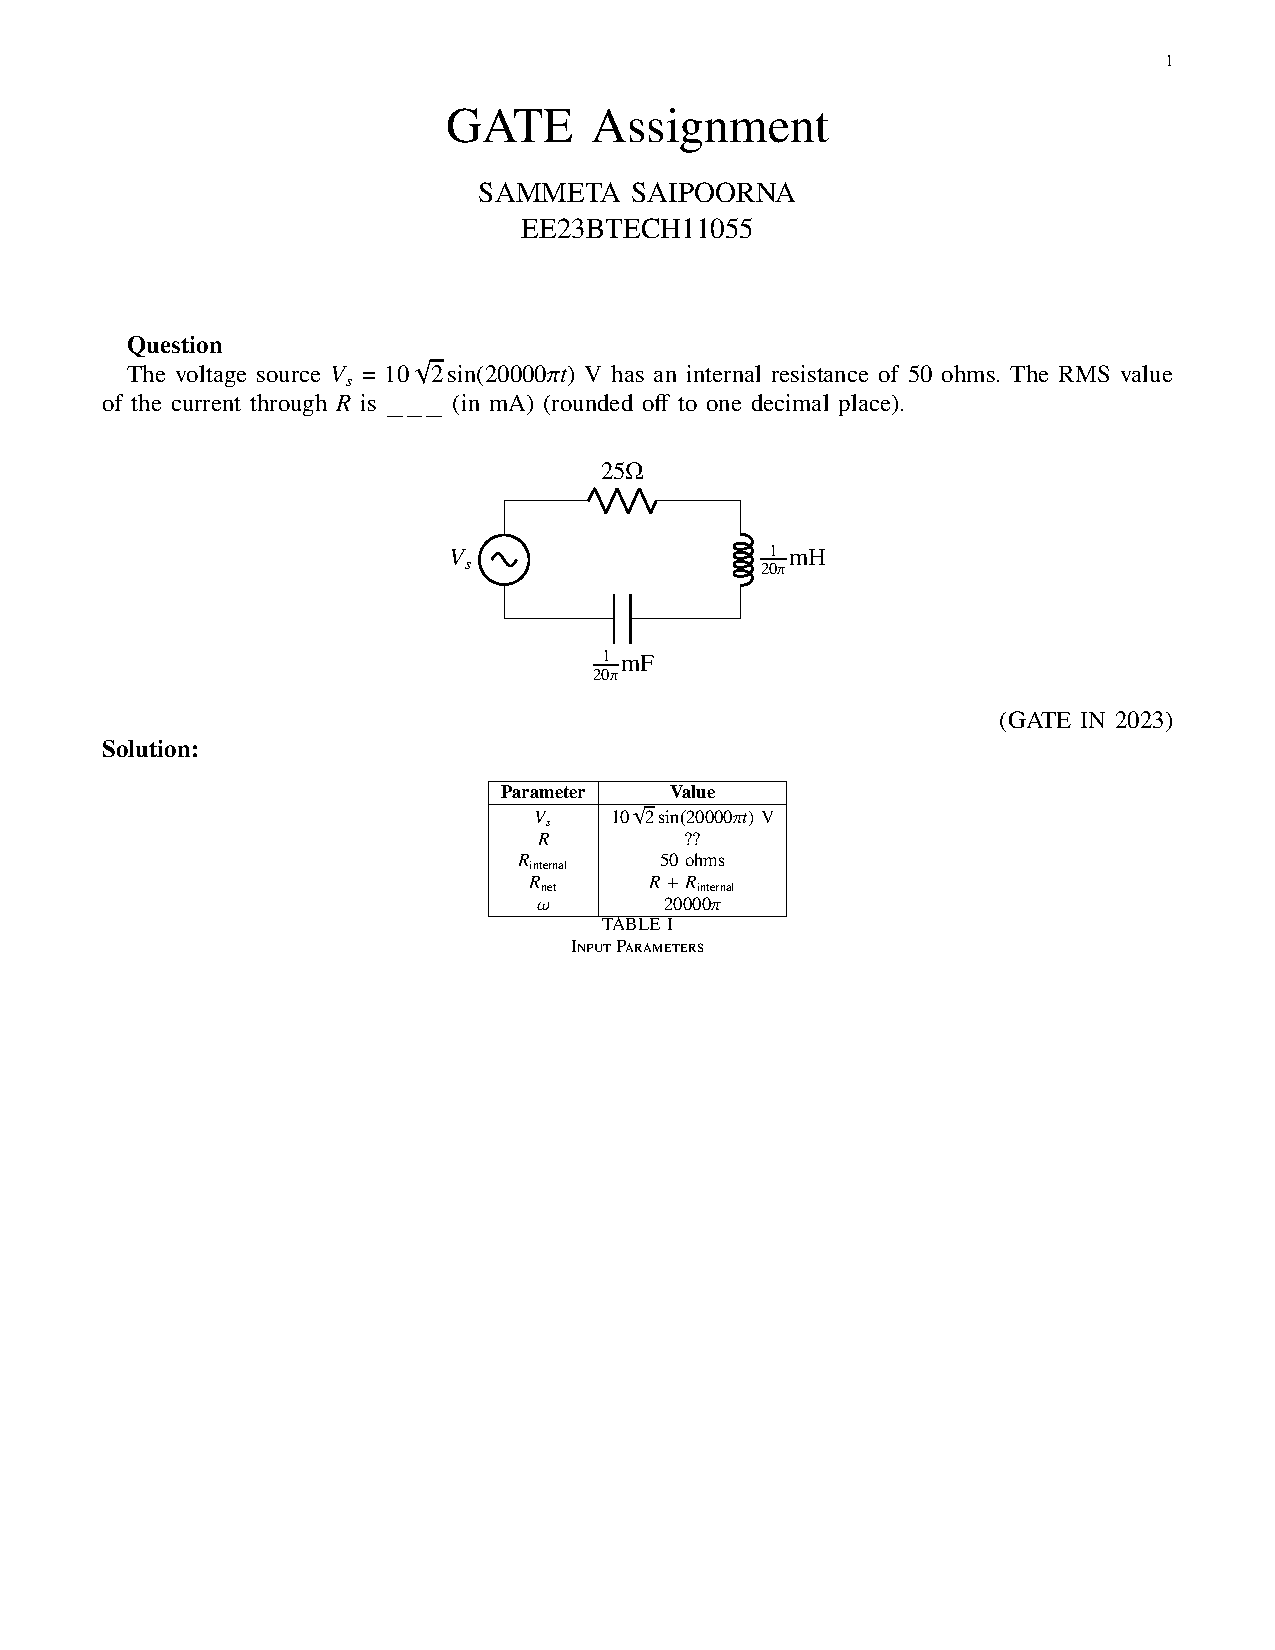
\includegraphics[width=1\linewidth]{2023/EC/35/figs/gate.png}
    \caption{ }
\end{figure}
\solution
\input{2023/EC/35/assign3.tex}
\pagebreak
\item A signal $x\brak{t}=2\cos{(180\pi t)}\cos{(60\pi t)}$ is sampled at 200 Hz and then passed through an ideal low pass filter having cut-off frequency of 100 Hz.\\
The maximum Frequency present in the filtered  signal in Hz is \rule{1cm}{0.5mm} (Round off to the nearest integer.) \hfill (GATE 2023 EE)
\solution
\input{2023/EE/63/main.tex}
\pagebreak
\item In the circuit shown, the input voltage $V_{in} = 100mV$. The switch and the opamp are ideal. At time $t=0$, the intial charge stored in the $10nF$ capacitor is $1nC$, with the polarity as indicated in the figure. The switch $S$ is controlled using a $1KHz$ square-wave voltage signal $V_s$ as shown. Whenever $V_s$ is `High', $S$ is in position $`1$' and when $V_s$ is `Low', $S$ is in position `$2$'.\\
At $t = 20ms$, the magnitude of the voltage $V_o$ will be  \\  
\begin{figure}[ht]
  \centering
    \resizebox{0.55\columnwidth}{!}{\input{2023/IN/60/figs/circuit1}}
\end{figure}
\hfill{(GATE IN 2023)}\\
\solution
\pagebreak

\item The value of parameters of the circuit shown in the figure are $R_1=2\ohm$,$R_2=2\ohm$,$R_3=3\ohm$,$L=10 mH$,$C=100\mu F$. For time \(t<0\), the circuit is at steady state with the switch $ 'K'$ in closed condition. If the switch is opened at $t=0$, the value of the voltage across the inductor \brak{V_L}
 at $t=0^{+}$ in Volts is \rule{2cm}{0.4pt} (Round off to 1 decimal place).
\begin{circuitikz}
    \draw (0,0) to [R, R=$R_3$] (0,2);
    \draw (0,3) to [switch, o-o, name=$K$] (0,2);
    \draw (0,3)-- (0,4);
    \draw (0,4) -- (4,4);
    \draw (3,0) to [american current source, l=$10\,\text{A,}\text{DC}$] (3,4);
    \draw (4,4) to (4,5) to (5,5) to[R, l=$R_1$] (6,5);
    \draw (6,5) to(7,5) to[L, l=$L$] (8,5) to (9,5);
    \draw (4,4)to (4,3)to (5,3) to[R, l=$R_2$] (6,3);
    \draw (6,3)to (7,3) to [C, l=$C$] (8,3) to(9,3);
    \draw (9,5) --(9,3);
    \draw (9,4) -- (10,4);
    \draw (10,4)-- (10,0);
    \draw(10,0)--(0,0);
\end{circuitikz} \hfill (GATE 2023 EE 29
Q)
\solution
\input{2023/EE/29/main.tex}
\pagebreak

\item The op amps in the circuit are ideal. The input signals are $V_{S1} = 3 + 0.10 \sin(300t), \text{V}$ and $V_{S2} = -2 + 0.11 \sin(300t)\, \text{V}$. The average value of the voltage $V_0$ is \underline{\hspace{1cm}} volts (rounded off to two decimal places).
\begin{figure}[ht]
\centering
\resizebox{0.55\columnwidth}{!}{\input{2023/IN/59/figs/gate.circuit.tex}}
\end{figure}
\hfill{(GATE IN 2023)}
\solution
\input{2023/IN/59/59.tex}
\pagebreak

\item The R-L circuit with $R=10 k\Omega$ and $L=1 mH$ is excited by a step current $I_0u(t)$. At $t=0^-$, there is a current $I_L=I_0/5$ flowing through the inductor. The minimum time taken for the current through the inductor to reach $99\%$ of its final value is $\ldots \mu s$
(rounded off to two decimal places).\\
\hfill{(GATE IN 2023)}
\solution
\input{2023/IN/47/main.tex}
\pagebreak


\end{enumerate}

